\titlespacing{\chapter}{0pt}{-50pt}{0pt}
\zihao{-4}
\chapter{引言}
\label{chap:introduction}
\section{选题背景与研究意义}
除了图像、视频,音频与自然语言处理等领域,人工智能(Artificial intelligence / AI)技术的快速发展也带动智能计算相关交叉学科的发展。AI助力的科学发现(AI for science / AI4Science)近年在计算生物、计算化学、新兴材料、计算天文,计算农业等都有广泛应用,相关AI技术的应用能够大幅加速相关科学研究进展。在计算制药领域,近年来相关AI技术在药物性质预测,设计,开发,实验等领域的运用不仅加速相关研究的进展,也能够降低相关研究的研发成本。人工智能在智能计算相关研究中开始扮演越来越重要的角色,相关模型在药物发现、药物属性预测等计算化学应用中已经展现出良好的性能和极大的潜力。由于深度学习技术应用具备为药物研发的多阶段降本增效的潜力,在2022年,AI制药赛道相关企业融资总金额达百亿美元。在这一赛道竞逐的有百度旗下的百图生科、华为EIHealth医疗智能体、深势科技,腾讯云深智药,还有初创企业晶泰科技,剂泰医药,星药科技等。相关成果已经展现出深度学习在该领域的强大性能和广阔前景。例如华为提出的盘古大模型已经具备在药物研发和临床诊断中实用的能力,深势科技提出了高精度的分子模拟计算模型和一站式药物计算设计平台。

基于AI的深度生成模型近十年来也被广泛研究,主流范式包括变分自编码器(Variational autoencoders / VAEs) \cite{vae_kingma_13},生成对抗模型(Generative adversarial networks / GANs) \cite{gan_goodfellow_14},流型模型(Normalizing flows / NFs) \cite{nice_dinh_15,density_dinh_17},自回归(Autoregressive models / ARs) \cite{ar_oord_16}与扩散模型(Diffusion) \cite{deepunsupervised_dickstein_15,generative_song_19}等。相关方法在图像生成,本文生成等方面也有了许多成功应用。

深度学习在计算化学领域近年来也有着诸多成功的实践。以分子学习为例,化学分子常以简化分子线性输入规范字符串(Simplified molecular-input line-entry system / SMILES) \cite{smiles_weinberger_88}的格式存储和计算,每一个分子式对应一个SMILES字符串。随着早期深度学习方法的出现与发展,诸如卷积神经网络(Convolutional neural networks / CNNs) \cite{cnnsmiles_hirohara_18}和循环神经网络(Recurrent neural networks / RNNs) \cite{rnnsmiles_bjerrum_17,practicalmodel_liu_19,deeppurpose_huang_20}等模型在图像和文本任务中展现出良好的表现。一些研究试图运用这些深度学习算法,对以字符串形式存储的分子式进行学习,以获得预测特定原子或是整个分子的性质的能力。随着图神经网络(Graph neural networks / GNNs) \cite{semisupervised_kipf_17,inductive_hamilton_17,howpowerful_xu_18}的出现,其对非结构化数据的建模能力和对节点间拓扑关系学习的能力被证明十分优异。分子作为自然界中天然存在的图结构,原子和键对应着图中的节点和边,这为分子学习提供了新的方法与范式。从最早的图卷积神经网络开始,相关研究致力于针对分子学习的典型特征,提出新的图学习算法,以提升对分子图学习的性能。随着相关化学模拟技术的发展,让三维分子建模成为可能。这也在拓扑结构信息以外,提供了更丰富的几何构型信息,这也驱动着相关研究拓展至几何图神经网络上。分子三维构象允许研究者对分子进行更准确的研究,同时也推动更多复杂任务的出现,包括分子设计,蛋白质配体(Ligand)设计,药物亲和力预测,蛋白质生成与性质等。

% 具体的任务包括药物分子设计,药物分子构象设计,蛋白质靶向嵌合体设计,蛋白质设计等,而本文聚焦的药物分子设计是其中的基础应用。本文的目标是提出一个能够批量设计具备特定性质药物分子的生成模型,相关成过能够帮助药物企业加快药物研发。同时,本文提出的模型具备对空间几何信息的优异学习能力,故将该模型也具备迁移至材料科学领域的潜力。

\section{国内外研究现状}
\subsection{基于深度学习的分子学习}
分子最早被表示为简化分子线性输入规范字符串,即SMILES字符串  \cite{smiles_weinberger_88},随着早期深度学习模型卷积神经网络和循环神经网络的发展,相关模型利用CNNs和RNNs对分子性质做出学习。Hirohara等 \cite{cnnsmiles_hirohara_18}的研究提出使用CNN对分子级别的特征和分子基团性质进行有效学习。由于RNNs在早期自然语言护理任务上有良好表现,Bjerrum \cite{rnnsmiles_bjerrum_17}提出LSTM-QSAR模型用于学习分子性质。

伴随图神经网络(GNNs)的发展,由于分子的形式天然的属于图结构,一些研究开始使用GNNs进行分子学习。CGCNN \cite{cgcnn_xie_18}将图卷积神经网络引入到分子性质学习,用以模拟并替代复杂的DFT计算。Xiong等 \cite{attentivefp_xiong_20}提出Attentive FP,一个结合注意力机制的图神经网络实现分子性质的有效学习与预测。GraSeq \cite{graseq_guo_20}提出在运用图神经网络学习拓扑结构同时,利用双向LSTM模型对SMILES分子式进行学习,通过两个通道联合预测分子性质。伴随相关技术的发展,研究者可以不再拘泥于原子拓扑结构,进而实现对分子三维结构的建模与学习。鉴于某一分子对应大量的同分异构体,而不同构象对应属性不尽相同,因此对三维构象的有效学习是十分必要的。EGNN \cite{egnn_satorras_21}在流行的图网络基础上,保留最基本的几何信息,即原子间距离,其简单的设计也成为了一些。在分子预训练框架GEM \cite{gem_fang_22}中,研究者提出GeoGNN图网络,将键长视作原子节点图的边特征,又对原子键构图,并将键角作为原子键图的边特征,通过在两个网络上的信息传递实现分子局部空间几何性质学习。Sch\"{u}tt等 \cite{schnet_schutt_17}在继承GNNs的信息传递范式的同时,将原子间距离用径向基函数(Radial basis funciton / RBF)建模后融入边特征,使算法对三维几何信息的有效学习的同时保证了等变性要求。SphereNet \cite{spherenet_liu_22}提出了基于球坐标系的信息传递范式SMP。通过一系列参考原子或键的规则,SMP在保证对原子对距离,键角和键扭转角这三个空间几何信息完整提取的同时,避免计算复杂度的爆炸式增长。ComENet \cite{comenet_wang_22}在ShpereNet的基础上,简化了空间几何信息的提取范式,在保证利用完整空间信息的前提下,以损失部分精度为代价,大幅度提升计算速度。

伴随着Transformer \cite{transformer_vaswani_17}相关研究在图像与文本领域的兴起,相关研究 \cite{smilestrans_honda_19,smilesbert_wang_19,chemberta_chithrananda_20}也利用Transformer对SMILES分子式进行学习。随着GTN \cite{gtn_yun_19}将Transformer引入图学习,越来越多的研究也将多头注意力机制用于分子图学习领域。大规模分子图预训练框架GROVER \cite{grover_rong_20}中,分子学习内核运用了GTransformer,同时学习分子中的原子与键的节点嵌入(embedding)或边嵌入。在分子预训练框架MPG \cite{mpg_li_21}中提出的图学习内核MolGNet放弃了对边嵌入的学习,仅利用多头注意力学习节点嵌入,结果证明了该图学习算法的有效性。

\subsection{基于深度生成模型的分子设计}
自深度学习研究兴起以来,深度生成模型一直是研究者重点研究的对象。作画、翻译、对话,渲染等应用能够直接服务于广大用户。主流的深度生成模型包括VAEs \cite{vae_kingma_13},GANs \cite{gan_goodfellow_14},NFs \cite{nice_dinh_15,density_dinh_17},ARs \cite{ar_oord_16}与Diffusion \cite{deepunsupervised_dickstein_15,generative_song_19}等。与图学习的演进过程相似,基于深度生成模型的分子设计也经历了从二维图结构到三维几何构象的演进。主流分子设计任务具体又可以被细分为:分子设计,分子优化,构象生成,蛋白质配体设计,蛋白质设计,蛋白降解靶向嵌合体设计等。

创新药物分子设计任务就是根据给定分子数据,使模型具备凭空生成全新且有效的药物分子图或三维结构。考虑到复杂药物分子主要由官能团等子结构组成,JT-VAE \cite{jtvae_jin_18}基于VAE生成树结构骨架,而后利用树结构骨架逐步生成分子图结构。GraphVAE \cite{graphvae_simonovsky_18}是早期的基于VAE的图生成研究,为避免离散化结构的线性表示的相关障碍,使其中解码器直接输出预设的最大概率的全连接图。基于NF模型,MoFlow \cite{moflow_zang_20}将隐式表征逐步映射到条件流过程中,模型首先生成连接原子的键,随后通过图条件流生成原子,并最终组成有效的分子图。

基于扩散模型的药物分子设计作为一个新兴的研究方向,此领域最早的研究为EDM \cite{edm_hoogeboom_22},其基于EGNN \cite{egnn_satorras_21}设计去噪过程内核,通过生成点云,再根据预设定的化学性质生成连接原子的键。MDM \cite{mdm_huang_23}在此基础上,提出了全新的去噪内核,通过两个SchNet \cite{schnet_schutt_17}分别对局部节点和全局节点特征进行学习。由于这种扩散模型更擅长在连续样本空间上的学习,故主流方法并不直接预测分子图中边的存在性,针对这一问题,DiGress \cite{digress_vignac_22}和MiDi \cite{midi_vignac_23}提出将图邻接矩阵引入扩散过程,并相应将马尔可夫状态转移矩阵引入噪声序列而非传统的高斯噪声。GCDM \cite{gcdm_morehead_23}针对对空间几何信息提取不足的问题,引入ColfNet \cite{colfnet_du_22}相似的空间几何学习范式,实现了对几何信息的充分学习。

\subsection{基于扩散模型的图生成模型}
在图学习领域中,一个图可以被表示为一个元组 $\mathcal{G} = (\mathcal{V}, \mathcal{E})$,其中包含了一个节点集合 $\mathcal{V}$ 和一个边集合 $\mathcal{E}$。在训练阶段,模型学习图在扩散过程中的概率分布,并被用于后续的采样阶段,以迭代地方式生成新的图。基于扩散的生成模型因其在多个领域的生成任务中表现出色而受到广泛关注,例如计算机视觉 \cite{blendeddiffusion_avrahami_22,cascadeddiff_ho_22,gradforshapegen_cai_20,sgmpointcloud_luo_21},自然语言处理 \cite{struccddpm_austin_21,argmaxflow_hoogeboom_21,stepunrolled_savinov_22},以及其他各种跨学科任务等 \cite{cdvae_xie_22,housediffusion_shabani_23,nap_lei_23}。

\begin{figure}[h]
  \centering
  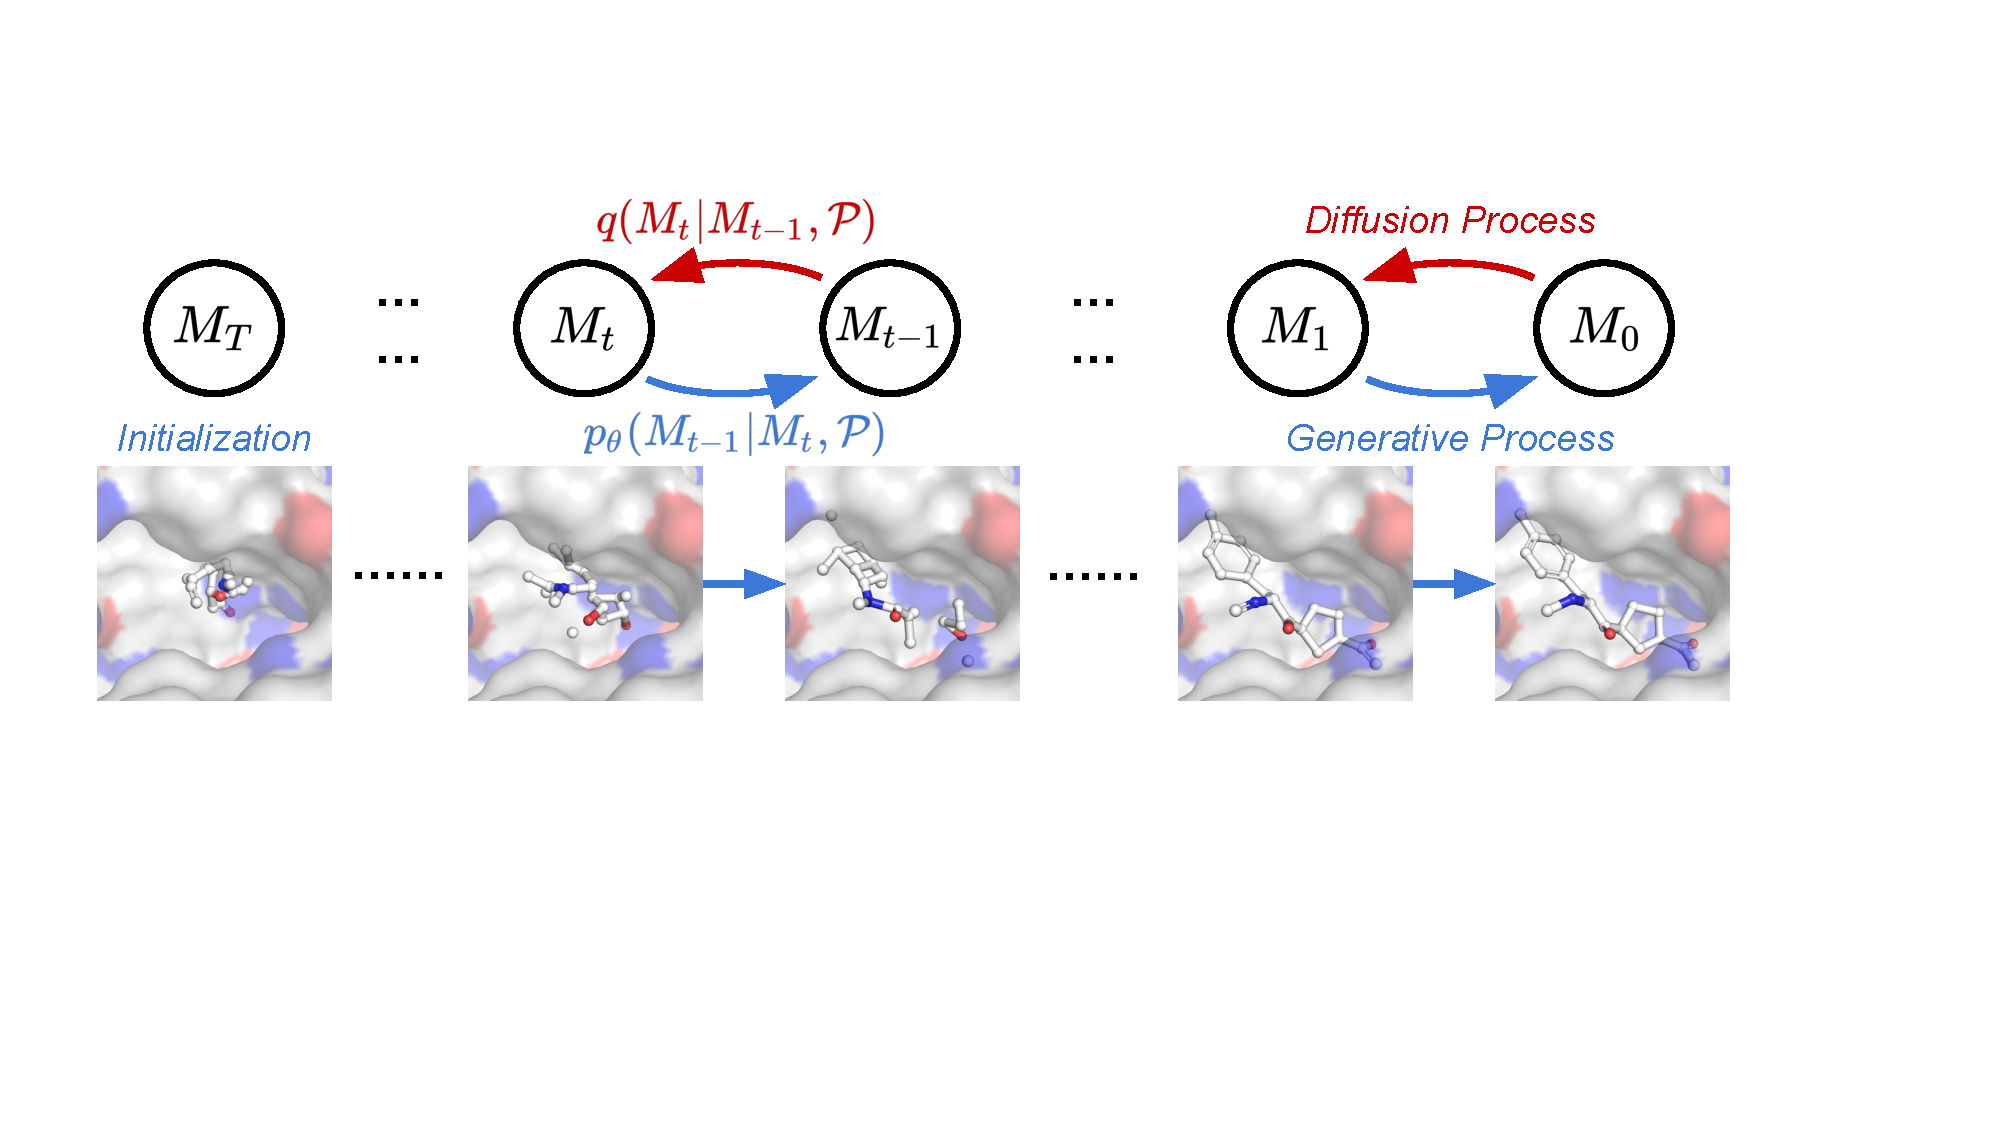
\includegraphics[width=\linewidth]{figures/targetdiff.pdf}
  \caption{基于扩散模型的分子生成的示意 \cite{targetdiff_guan_23}}
  \label{fig:targetdiff}
\end{figure}

除去创新药物分子设计这一子领域,扩散模型在计算化学和计算医药领域也有其他广泛应用。图~\ref{fig:targetdiff}~是一个基于扩散模型的分子生成模型的典型范式的示意。分子构象生成要求根据给定的分子式,生成对应的三维分子构象。由于不要求对边的形成进行建模,故这也是一个较为简单的任务。ConfGF \cite{confgf_shi_21}是最早将扩散模型引入构象生成的模型,该模型学习原子坐标的对数似然的梯度场,并将其视作作用在原子上的赝力,随后根据朗之万动力学采样生成样本。于其他对原子坐标进行扩散/去噪的范式不同,Torsion Diffusion \cite{tordiff_jing_22}仅通过对扭转角进行建模实现对分子构象的预测,这一范式极大减小了采样空间的大小。该方法提出了一个显式到隐式的得分模型,将三维显式坐标转换为扭转角空间上的隐式得分。最终,分子构象通过一个Boltzmann生成器预测。在更下游的任务中,一些研究致力于研究蛋白质靶向嵌合体生成,即在给定蛋白质靶点的条件下,生成能够与之稳定连接的药物分子。先前基于其他ARs \cite{graphbp_liu_22, arligand_luo_21, pocket2mol_peng_22}的研究以序列的方式生成配体,这可能导致对全局多体交互信息提取不充分与不一致以及生成过程的早停现象。针对这一缺陷,DiffBP \cite{diffbp_lin_22} 提出了一个靶点感知的扩散模型并直接生成完整的蛋白质配体。尽管该方法显著提升了生成样本的有效性,但在子结构的药物特性方面仍存在欠缺。TargetDiff \cite{targetdiff_guan_23}提出了一个SE(3)等变的GNN去噪内核,将生成模型与嵌合体的结合亲和力排序联系起来,用于评价生成样本的特性。该方法被证明能够通过无监督的方式提升药物和靶标的结合亲和力。

\begin{figure}[h]
  \centering
  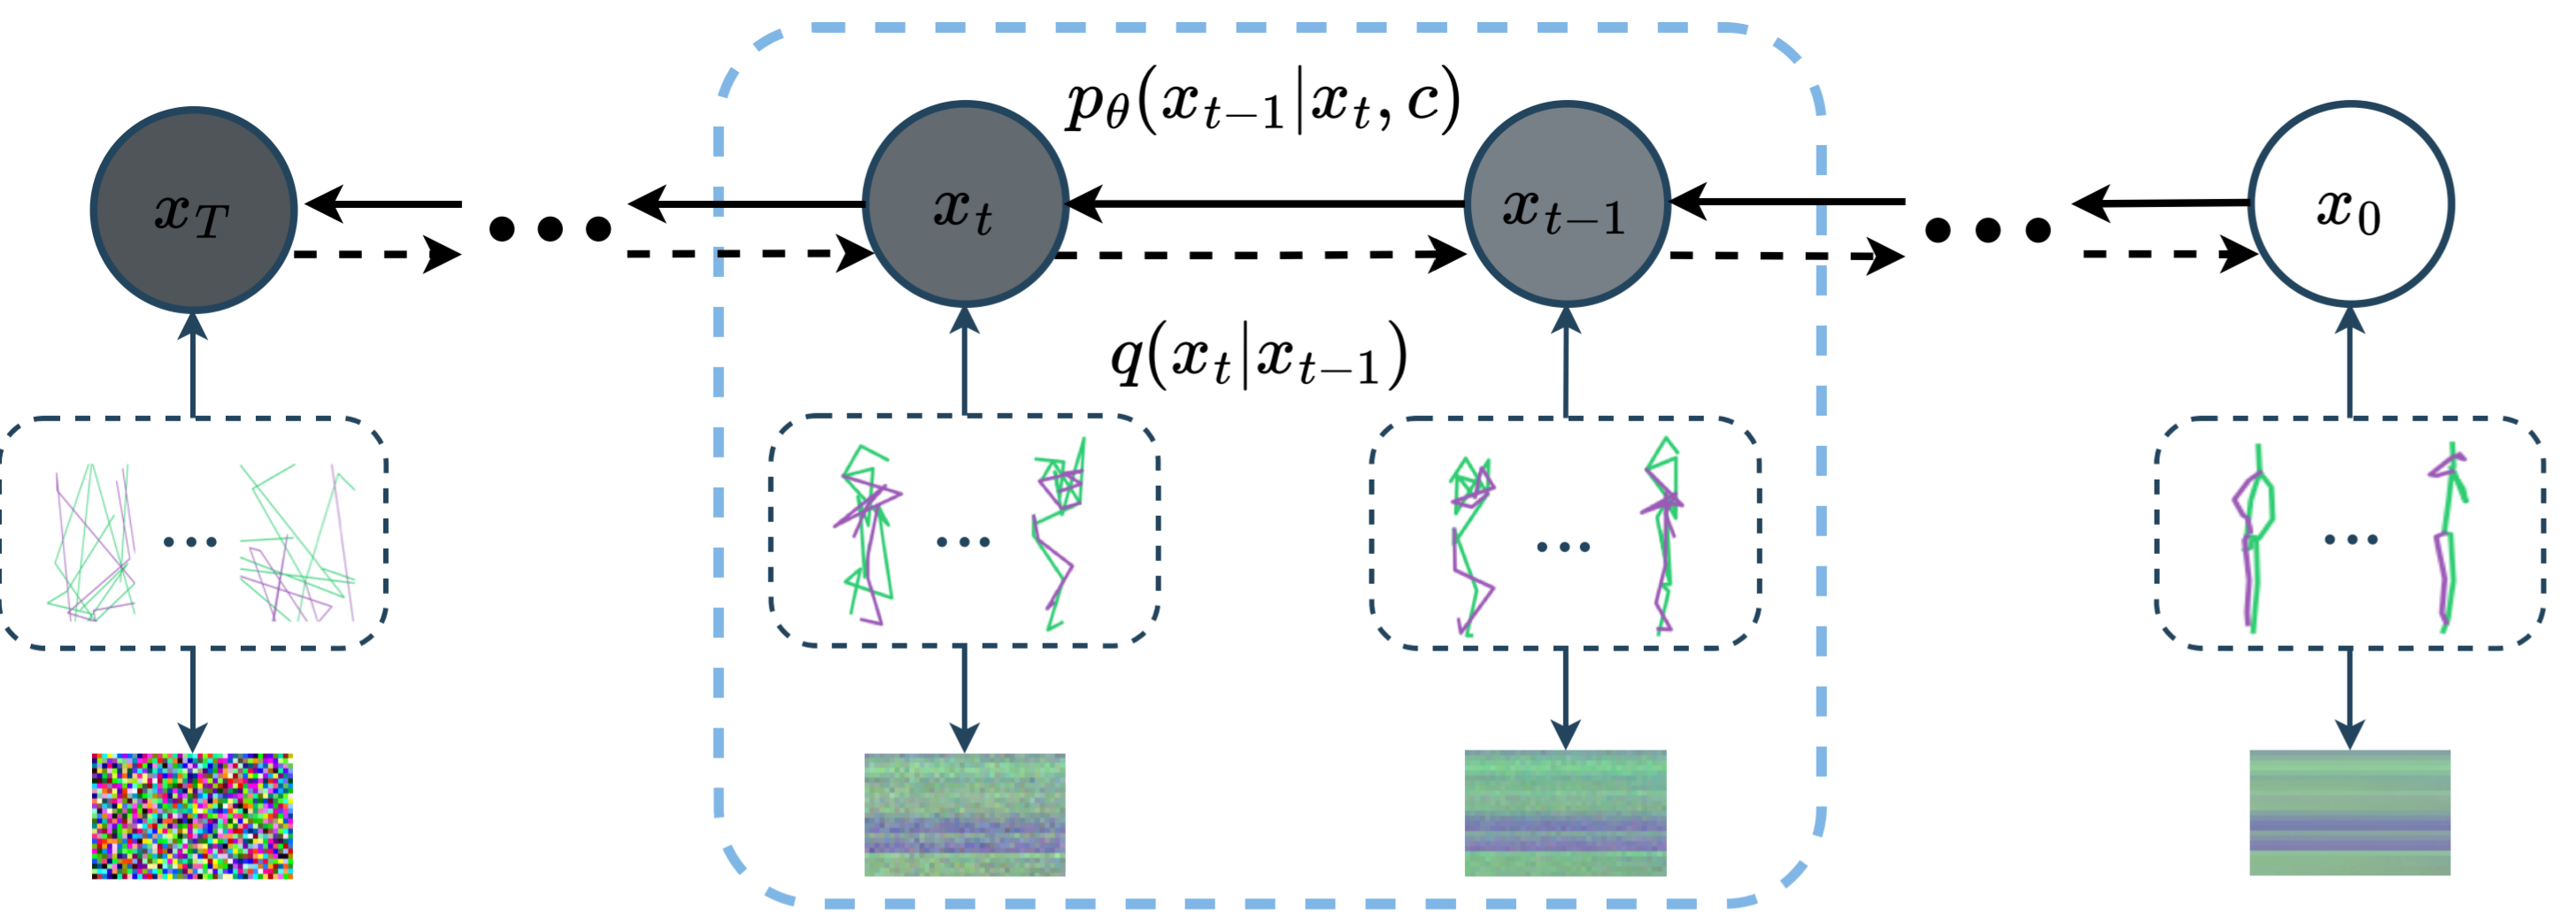
\includegraphics[width=\linewidth]{figures/modiff.png}
  \caption{基于扩散模型的人体动作生成的示意 \cite{modiff_zhao_23}}
  \label{fig:modiff}
\end{figure}

人体骨架的表示形式与分子类似,都是表示为在三维空间内被边连接起的点云。不同之处在于生成人体骨架动作时,不需要对边的存在性进行预测。图~\ref{fig:modiff}~是一个基于扩散模型的人体动作生成的典型范式示意。MoFusion \cite{mofusion_dabral_22}在人体动作生成中使用U-Net \cite{unet_ronneberger_15}作为扩散模型中去噪核心的架构。MoDi \cite{modi_raab_22} 利用结构感知神经滤波器和3D卷积,实现对每个关节的精确控制。

除了在分子设计和人体动作生成上的应用外,许多研究工作致力于将扩散过程用于一般形式的图拓扑结构生成。SaGess \cite{sagess_limnios_23}通过引入广义分治框架来增强DiGres \cite{digress_vignac_22}在图生成任务中的表现。对于图拓扑结构生成,EDP-GNN \cite{edpgnn_niu_20}将Score SDEs结合到离散图邻接矩阵生成中。在此基础上,GraphGDP \cite{graphgdp_huang_22}提出了名为Position-enhanced图得分网络的去噪核心,以实现对位置信息的进一步利用。GSDM \cite{gsdm_luo_22}不仅仅在边属性上进行采样,还利用了节点特征和图谱空间上的Score SDE高效地生成图,这在通用数据集和分子数据集上得到了验证。受VAEs启发,NVDiff \cite{nvdiff_chen_22}采用变分图自编码器(VGAE)结构,首先对图在隐变量空间上的特征进行采样,然后将其解码为节点或边特征。EDGE \cite{edge_chen_23}将扩散模型引入大图生成,扩散过程中逐渐移除边,直到图为空。该模型还通过仅关注部分节点来避免生成过多的边。专为双曲图设计的HGDM \cite{hgdm_wen_23}在提取双曲嵌入的复杂几何特征方面表现出优良的性能。

\begin{figure}[h]
  \centering
  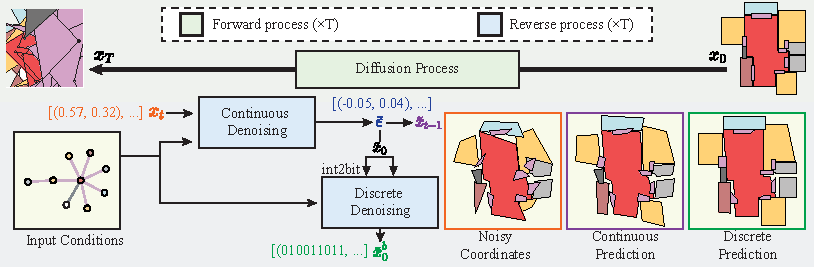
\includegraphics[width=1.0\linewidth]{figures/housediffusion.pdf}
  \caption{HouseDiffusion模型框架示意 \cite{housediffusion_shabani_23}}
  \label{fig:housediffusion}
\end{figure}

除了在图的拓扑结构生成上的基础研究,有一些研究进一步将扩散模型引入实际的图数据生成的应用中。HouseDiffusion \cite{housediffusion_shabani_23}将基于扩散的图生成引入户型设计领域。该方法将房间视为图中节点,将门视为连接节点的边。每个节点都由一个2D坐标序列环组成,序列中的每个坐标代表着房间角落所处的位置。实验结果显示模型能够生成精确且多样的户型。图~\ref{fig:housediffusion}~为HouseDiffusion的模型框架示意。

\begin{figure}[h]
  \centering
  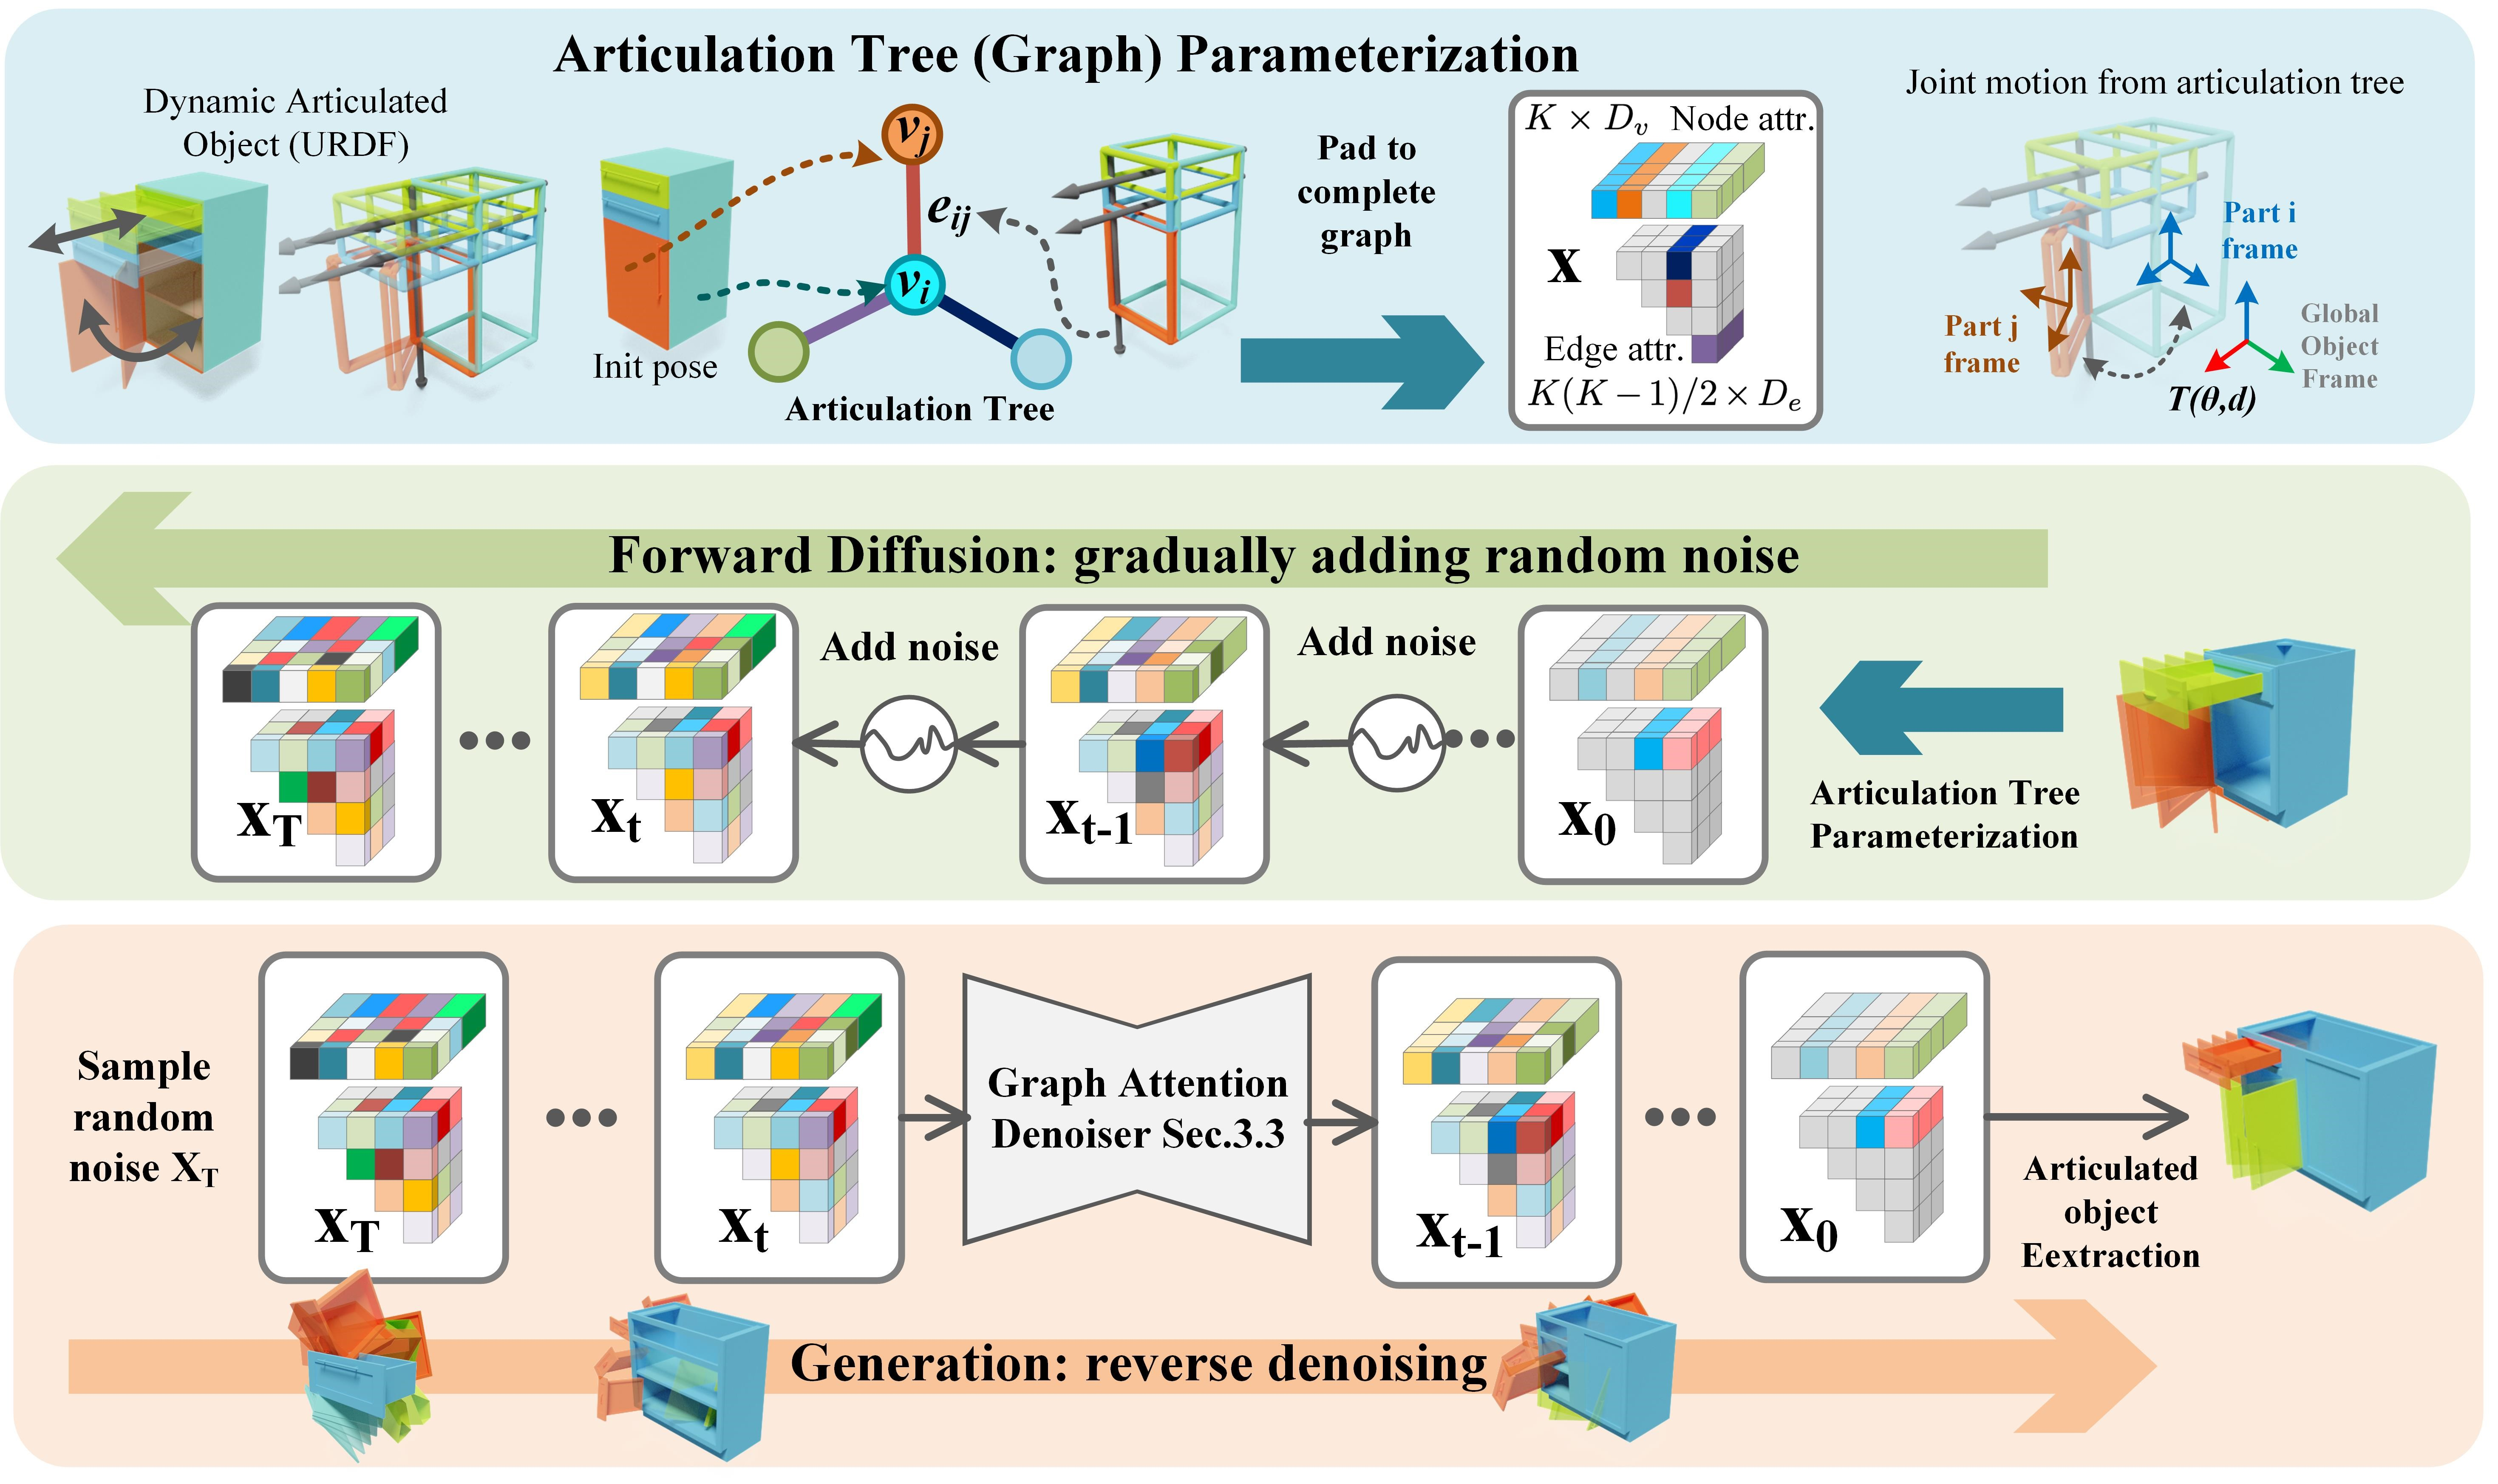
\includegraphics[width=1.0\linewidth]{figures/nap.jpg}
  \caption{NAP模型框架示意 \cite{nap_lei_23}}
  \label{fig:nap}
\end{figure}

NAP \cite{nap_lei_23}将基于扩散的图生成方法用于铰接体生成,图~\ref{fig:nap}~为其结构示意。该方法将铰接体中的子结构视为节点,将各子结构间的旋转或是抽拉的几何关系视为节点间的边。NAP基于DDPM,构建铰接体树结构,并通过采样节点和边特征,生成3D铰接体。为了更好促进的阿尔茨海默病等疾病诊断,Brain Diffuser \cite{braindiffuser_chen_23}利用扩散模型,根据大脑张量图片生成对应的大脑网络结构。 Lu等人 \cite{modeling_lu_23}提出模拟离散扩散模型,利用节点特征生成创新的仿生蜘蛛网结构及类似物。Diff-POI \cite{diffpoi_qin_23}对用户局部偏好进行采样,并将其用于兴趣点推荐。

\section{研究内容}
近年来,深度生成模型,特别是基于扩散模型的生成模型 \cite{ddpm_ho_20,sgm_song_19,scoresde_song_21}在各个生成式人工智能研究领域中都取得了广泛且重大的进展。与生成方法的发展趋势相一致,分子发现领域的主流方法已经从之前的生成模型转变为基于扩散的模型,并从设计2D图形转变为3D构象。然而,创新三维药物分子设计面临两个主要挑战。第一个挑战是在预测准确稳定的分子构象方面,而另一个挑战则是充分利用几何信息以促进离散图结构的生成。在本文中,我们提出了几何促进的分子扩散(Geometric-facilitated Molecular Diffusion / GFMDiff),这是一种解决上述挑战的全新的3D药物分子设计方法。GFMDiff能够生成准确的3D几何构型,同时解决图自身离散性带来的诸多问题。

作为扩散模型中广泛采用的范式,去噪扩散概率模型(Denoising Diffusion Probabilistic Models / DDPMs) \cite{ddpm_ho_20,dpm_jascha_15}在各种生成任务中表现出色。通过在前向过程中逐渐添加高斯噪声,将输入数据转换为预定义的噪声分布,并在采样阶段迭代去噪,最终得到生成结果。与VAEs \cite{vae_kingma_13}和GANs \cite{gan_goodfellow_14}等端到端方法相比,这种在每个时间步训练扩散模型的方法在准确性、效率和训练难度方面表现更好。扩散模型在计算化学 \cite{edm_hoogeboom_22,targetdiff_guan_23}和生物学 \cite{diffab_luo_22,protseed_shi_23}等领域的应用已经显示出卓越的性能。在药物分子设计任务的背景下,逐步调整分子构象与分子动力学的核心原理高度一致。

创新药物分子设计是分子生成领域一个重要的任务,该任务要求生成有效、新颖且结构稳定的分子。为了解决生成的3D构象所要求的等变性条件,一些基于扩散的方法 \cite{edm_hoogeboom_22,mdm_huang_23}通过原子间距离间接对分子进行建模,这直接反映了原子间相互作用力的强度。然而,早期的方法 \cite{edm_hoogeboom_22}没有解决多个原子之间的复杂原子间关系。而MDM \cite{mdm_huang_23}只是简单地使用阈值区分化学键和原子间力所造成的影响,而不考虑具体的原子和键的类型。最近的研究 \cite{moleformer_yuan_23}表明,键角之于分子学习与原子对间相互距离同样重要,但只有少数方法充分利用了空间信息。此外,由于分子扩散方法只作用于点云,传统的图卷积无法区分不同原子的重要性。鉴于这些挑战,我们设计了一种新颖的双轨分子学习框架,命名为双轨Transformer网络(Dual-track Transformer Network / DTN)。通过集成全局Transformer架构,本文将DTN作为扩散模型的去噪核函数,实现对空间几何信息的充分学习。

在分子生成领域,基于自回归模型(ARs)\cite{gschnet_wallach_19,gshperenet_luo_22},流型模型(NFs)\cite{moflow_zang_20,graphaf_shi_20}和变分自编码器(VAEs)\cite{jtvae_jin_18,cgvae_liu_18}等方法已经有了一些成功尝试。鉴于扩散模型在连续数据上的出色性能,大多数分子图生成模型采用了在笛卡尔坐标和特征上采用扩散和去噪方法,然后基于预定义的规则生成分子图,而不是直接通过模型预测键的存在。间接生成图形的方式可能导致生成样本的稳定性和有效性有所下降。为了使扩散模型适用于分子的多模态数据,一些研究 \cite{edpgnn_niu_20,digress_vignac_22,midi_vignac_23}在扩散和去噪过程中引入了邻接矩阵。然而,将图和边嵌入模型中会导致计算成本的增加。在我们的研究中,我们将扩散模型视为一个过程,即在每个时间步根据局部多体原子间关系逐步更新原子信息。准确的特征学习有助于对分子构型进行精确预测。为了预测准确的分子构象,我们设计了一种在训练过程中减少嵌入和局部几何之间差距的方法。在本文中,我们通过精心设计的损失函数几何促进的损失函数(Geometric-facilitate Loss / GFLoss),在训练过程中积极的干预模型学习,促使模型生成稳定且合理的化学键。

在实验部分中,本文测试了GFMDiff在药物分子设计任务上,和去噪内核DTN在分子性质预测任务上的表现。在药物分子设计任务中,本文在GEOM-QM9 \cite{qm9_ramakrishnan_14}和GEOM-Drugs \cite{drugs_axelrod_22}上测试了GFMDiff和时下最优的基线模型的性能,并进行消融实验验证了GFMDiff各创新模块的有效性。同时,为进一步检验去噪内核DTN对空间几何信息的提取能力,本文在GEOM-QM9和OC20 \cite{oc20_chanussot_21}数据集上对比了DTN和时下最优的几何图神经网络在分子性质预测任务上的性能。结果显示,本文的GFMDiff是时下表现最好的创新药物分子设计模型,同时DTN也在多个基准测试中证明了其对几何图结构的优异学习能力。

\section{创新点}
在本文中,我们提出了用于创新药物分子设计的几何促进的分子扩散(Geometric-facilitated Molecular Diffusion / GFMDiff)框架。与先前的方法主要基于原子对距离学习原子特征不同,本文成功地将三元几何信息与原子对距离有效地结合到分子学习中。本领域大多数研究在生成式直接生成点云,并根据预设规则完成3D图结构的搭建。然而这种方法存在两个主要问题。首先,间接的图生成方式导致样本的稳定性和有效性下降。其次,传统的图卷积不足以区分局部和全局信息。为了解决第一个约束,本文设计了一个精巧的几何促进的损失函数(Geometric-facilitate Loss / GFLoss),在训练阶段主动引导键的形成。至于第二个约束,我们引入了双轨Transformer网络(Dual-track Transformer Network / DTN),这是一个基于全局Transformer的神经网络,以促进全面的几何学习和局部特征学习。最后在试验阶段,本文进一步在分子性质预测任务上检验了本文提出的DTN神经网络的有效性。总而言之,本文的创新点如下:

$\bullet$ 本文提出的GFMDiff框架及其中的DTN网络,能够综合且全面的利用空间信息,以捕捉原子之间的多体相互作用,这对生成有效且稳定的全新分子至关重要。

$\bullet$ 为了解决图形的离散性问题,引入了一个精心设计的GFLoss,以促进键的形成,并以高效的方式处理由图内在离散性与扩散模型不兼容带来的挑战。

$\bullet$ 提出了DTN作为全局图卷积的替代方案,可以有效地捕捉全局和局部信息,并在后续的分子性质预测任务中进一步验证其有效性。

\section{基本框架}
\begin{figure}[h]
    \centering
    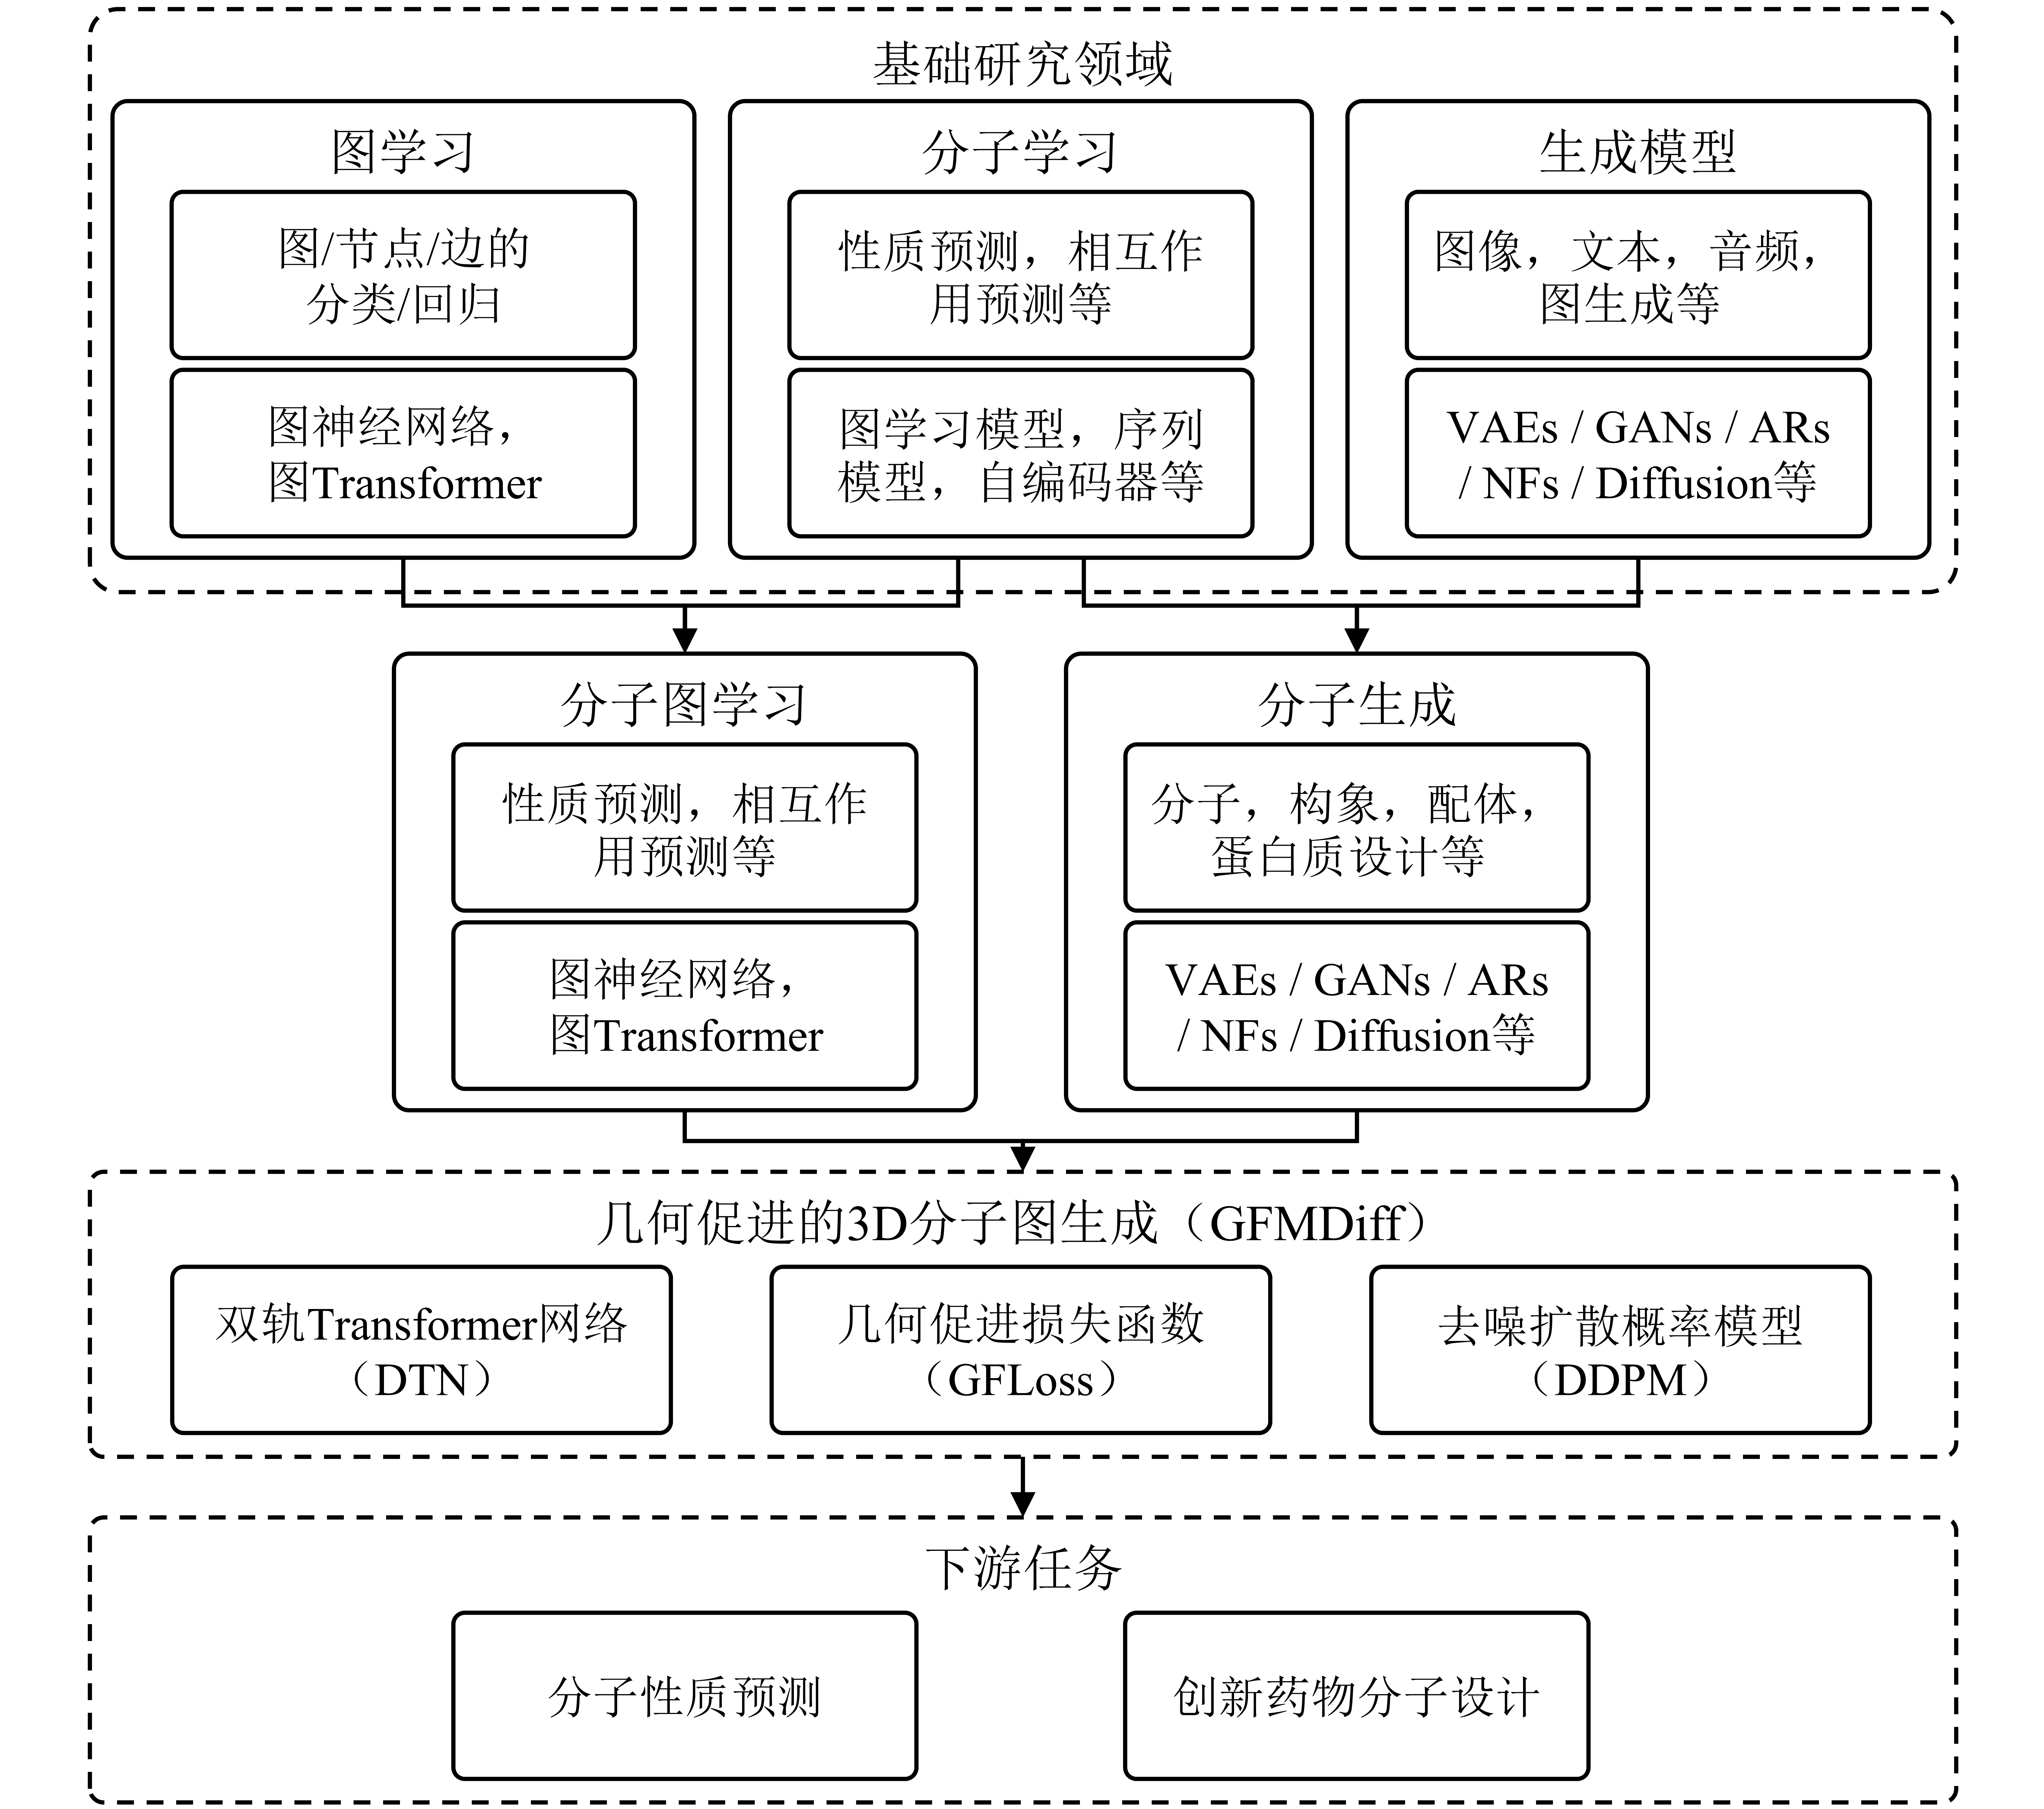
\includegraphics[width=\linewidth]{figures/overall_structure.png}
    \caption{本文总体框架示意}
    \label{fig:oa_struc}
  \end{figure}

在图~\ref{fig:oa_struc}~中,本文展示了本文的总体框架。在图学习,分子学习和生成模型这三个基础研究领域的基础上,出现了分子图学习和分子生成这两个交叉研究领域。本文提出的几何促进的3D分子图生成(GFMDiff)模型基于扩散模型中的去噪扩散概率模型(Denoising diffusion probabilistic models / DDPMs),构建了双轨Transformer网络作为去噪内核。同时,为了实现更好的药物分子设计性能,本文提出了GFLoss损失函数项。本文的GFMDiff模型能用于作药物分子设计的下游任务,同时DTN也能被用作分子性质预测下游任务。本文可分为五章,每章的主要内容如下:

第一章为引言,本文在该部分介绍了药物分子设计的研究背景及意义,以及分子学习,分子设计和扩散模型等相关研究领域的研究现状。随后,本文阐述了现有基于扩散的药物分子设计面临的主要问题,针对性的解决方法和本文主要创新点。

第二章为理论介绍,本文在该部分介绍了基于图神经网络和Transformer的分子图学习范式,几何神经网络的等变性要求和基于扩散的生成模型等理论知识。

第三章为方法论,本文在该部分介绍了本文提出的GFMDiff框架,包括其中的DTN去噪内核,GFLoss损失函数及相关训练过程。

第四章为实验,本文在该部分介绍了本文的GFMDiff模型在两个公开数据集的三个药物分子设计任务中的表现,并将其与时下最前沿的相关模型对比。同时,本文也通过消融实验检验了本文提出的各个创新模块的有效性。此外,为充分衡量去噪核心DTN在分子学习中的能力,本文检验了其在两个公开数据集上的分子性质预测任务的表现。

第五章为总结与展望,本文首先在该部分总结了本文的主要创新和取得的成果,而后对药物分子设计和图生成模型的未来发展做出展望。